\documentclass[letterpaper, 10 pt, conference]{ieeeconf}
\IEEEoverridecommandlockouts % This command is only needed if
% you want to use the \thanks command

\overrideIEEEmargins % Needed to meet printer requirements.

% See the \addtolength command later in the file to balance the column
% lengths on the last page of the document
\usepackage{microtype}
% The following packages can be found on http:\\www.ctan.org
% \usepackage{graphics} % for pdf, bitmapped graphics files
% \usepackage{epsfig} % for postscript graphics files
% \usepackage{mathptmx} % assumes new font selection scheme installed
% \usepackage{times} % assumes new font selection scheme installed
% \usepackage{amsmath} % assumes amsmath package installed
% \usepackage{amssymb} % assumes amsmath package installed

\usepackage[pdftex,pdfauthor={Michael Everett},pdftitle={6.867 Pset 1}]{hyperref}
\hypersetup{colorlinks,linkcolor={green!50!black},citecolor={green!50!black},urlcolor={blue!80!black}}
\makeatletter \let\NAT@parse\undefined \makeatother
% \usepackage[square,comma,sort&compress]{natbib}
\usepackage[sort,compress]{cite}
\usepackage{graphicx} % more modern
\usepackage{amsfonts}
\usepackage{amsmath,soul}
\usepackage{color}
\usepackage[font=small]{subcaption}
\usepackage{balance}
\usepackage[font=small]{caption}
%\usepackage{subfigure,balance}
%\usepackage[colorlinks=true]{hyperref}
%\usepackage{subcaption,balance}
%\usepackage{algorithm} \usepackage[noend]{algorithmic}
\usepackage[linesnumbered,ruled,vlined]{algorithm2e}
\usepackage{multirow}

\DeclareMathOperator*{\argmin}{\arg\!\min}
\DeclareMathOperator*{\argmax}{\arg\!\max}
\usepackage{tabulary}
\newcolumntype{K}[1]{>{\centering\arraybackslash}p{#1}}


\newtheorem{definition}{Definition}
\newtheorem{assumption}{Assumption} \newtheorem{theorem}{Theorem}
\newtheorem{lemma}{Lemma}
\newtheorem{corollary}[theorem]{Corollary}

\title{\LARGE \bf 6.867 : Homework 1}

\author{Anonymous authors}

% \usepackage[usenames]{color}
%\DeclareMathOperator*{\argmin}{arg\,\!min}
%\DeclareMathOperator*{\argmax}{arg\,\!max}
\usepackage[svgnames]{xcolor} \definecolor{DarkGreen}{rgb}{0,0.5,0}
\definecolor{DarkRed}{rgb}{0.75,0,0}

\usepackage[authormarkuptext=name,addedmarkup=bf,authormarkupposition=left]{changes}
%\usepackage[final]{changes} %Use this to hide all comments.
\definechangesauthor[name={M.~E.}, color={red}]{me}
\setremarkmarkup{(#2)}

%\newcommand{\mXX}[1]{{\color{DarkRed} \bf XX #1 XX\ }}
\newcommand{\mXX}[1]{\added[id=ml,remark={}]{#1}}
\newcommand{\sXX}[1]{\added[id=sc,remark={}]{#1}}
%\newcommand{\XX}[1]{{\bf \color{red} XX #1 XX}}
\newcommand{\XX}[1]{\added[id=jh,remark={}]{#1}}
\newcommand{\jmXX}[1]{\added[id=jm,remark={}]{#1}}
\newcommand{\meXX}[1]{\added[id=me,remark={}]{#1}}



\newcommand{\jsec}[1]{\marginpar{\fcolorbox{yellow}{yellow}{\parbox{0.7in}{\raggedright
        \color{blue} \tiny #1 }}}}
\newcommand{\hsec}[1]{\marginpar{\fcolorbox{yellow}{yellow}{\parbox{0.7in}{\raggedright
        \color{green} \tiny #1 }}}}
\newcommand{\jhmargin}[2]{{\color{orange}#1}\marginpar{\color{orange}\tiny\raggedright
    \bf [JH] #2}}


\usepackage{tikz,mathtools}
%\usepackage{cleveref}
\usepackage[capitalize]{cleveref}
\crefformat{equation}{(#2#1#3)}
\Crefformat{equation}{Equation~(#2#1#3)}
\Crefname{equation}{Equation}{Equations}

\newcommand{\inputTikZ}[2]{\scalebox{#1}{\input{#2}}}
\usetikzlibrary{shapes,positioning,automata,arrows,fit,backgrounds,calc}
\tikzstyle{block} = [draw, fill=blue!20, rectangle,minimum height=1em,
minimum width=2em] \tikzstyle{sum} = [draw, fill=blue!20, circle, node
distance=1cm] \tikzstyle{input} = [coordinate] \tikzstyle{output} =
[coordinate] \tikzstyle{pinstyle} = [pin edge={to-,thin,black}]
\usetikzlibrary{trees} \usetikzlibrary{decorations.pathmorphing}
\usetikzlibrary{decorations.markings}
\definecolor{darkgreen}{rgb}{0,0.5,0}
\definecolor{darkred}{rgb}{220,20,60}

\makeatletter
\renewcommand\paragraph{\@startsection{subsubsection}{4}{\z@}%
{0.25ex \@plus.5ex \@minus.2ex}%
{-.15em}%
{\normalfont\normalsize\itshape}}
\makeatother


\begin{document}

\maketitle
\thispagestyle{empty} \pagestyle{empty}

% %%%%%%%%%%%%%%%%%%%%%%%%%%%%%%%%%%%%%%%%%%%%%%%%%%%%%%%%%%%%%%%%%%%%%%%%%%%%%%%
% \begin{abstract} 
% Abstract here.
% \end{abstract}

%%%%%%%%%%%%%%%%%%%%%%%%%%%%%%%%%%%%%%%%%%%%%%%%%%%%%%%%%%%%%%%%%%%%%%%%%%%%%%%%
%!TEX root = main.tex
\section{Neural Networks} \label{sec:prob1}
In this problem, we implement a simple neural network in Python.
The network is trained with backpropogation and stochastic gradient descent.

\subsection{Part 1}
In this problem, we are mainly interested in classification tasks.
Thus, we pass the output of the final hidden layer through a softmax layer to generate a probability (outputs are positive and sum to 1) vector where each element $k$ is the probability of the input being in class $k$.

In general, the training objective is to minimize loss, so at each training step, we evaluate the loss function and compute its gradient, and then adjust the weights and biases in a direction to decrease loss according to the learning rate.
According to the backpropogation algorithm, the derivative of loss with respect to final activation is $\delta^L = Diag[f'(z)] \nabla_a loss$.
For this network with softmax output activation and cross-entropy loss function, we can compute $\delta^L = p(x) - y$, where p(x) is the predicted output for a particular training data point, $x$ in class $y$ (where p is also a function of the network weights, and other parameters).


\subsection{Part 2}
According to the Xavier Initialization, we can initialize weights to be a zero-mean Gaussian with variance [todo].
We initialize biases to zero, but if we initialize weights to zero as well, [todo].

\subsection{Part 3}
To add weight regularization, the objective function would look like:
\begin{equation}
J(w) = l(w) + \lambda(||w^{(1)}||^2_F + ||w^{(2)}||^2_F)
\end{equation}
The only change to the pseudo-code from the lecture notes would be an updated gradient term.
[todo]: gradient term.






\section{MNIST Dataset} \label{sec:prob4}
In this section, we use each of the algorithms to classify handwritten digits from the MNIST dataset.

\subsection{Part 1}
The MNIST dataset contains labeled, handwritten digits.
We split the dataset into multiple classification tasks, shown in the first column of~\cref{table_4_1}.
We also split it into training, validation, and testing sets.

We follow the typical procedure: train with many hyperparameters (C for $L_1$, $L_2$ for LR, and C for SVM), choose the hyperparameters that maximize performance on the validation set with lowest model complexity (low C), and report performance on the test set for the best hyperparameters.

The two classifiers here, Logistic Regression and Linear SVM, perform similarly on each classification task.
For all tasks, the training accuracy was better than the testing accuracy, as expected.

Normalization of the data did not make a large difference ($<\pm 1\%$) for these classifiers, and results presented are for non-normalized data.
The only significant difference after normalization was the size of regularization constant $C$; in all cases, normalization caused the optimal $C$ value to increase by a few orders of magnitude.
This is likely because the size of the data elements decreased, so the size of the learned weight vector increased, meaning a smaller regularization cost had to be applied for the same effect.

A couple misclassified digits are shown in~\cref{fig:misclassified}.
Some handwriting is very difficult even for humans to classify, so it makes sense that our learned classifiers are not perfect.

\begin{figure}\label{fig:misclassified}
    \centering
    \begin{subfigure}[b]{0.5\columnwidth}
        \centering
        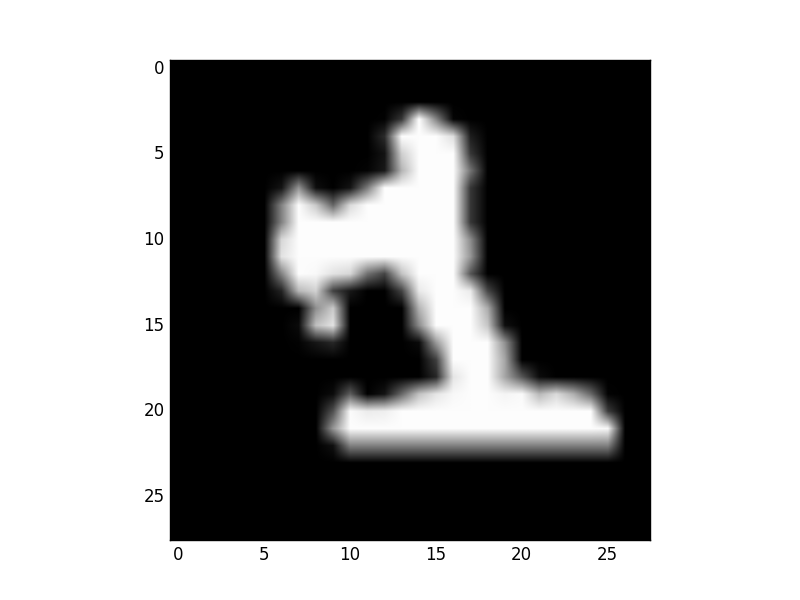
\includegraphics[height=1.2in]{figures/4_1_bad1}
        \caption{Misclassified 1}
    \end{subfigure}%
    ~ 
    \begin{subfigure}[b]{0.5\columnwidth}
        \centering
        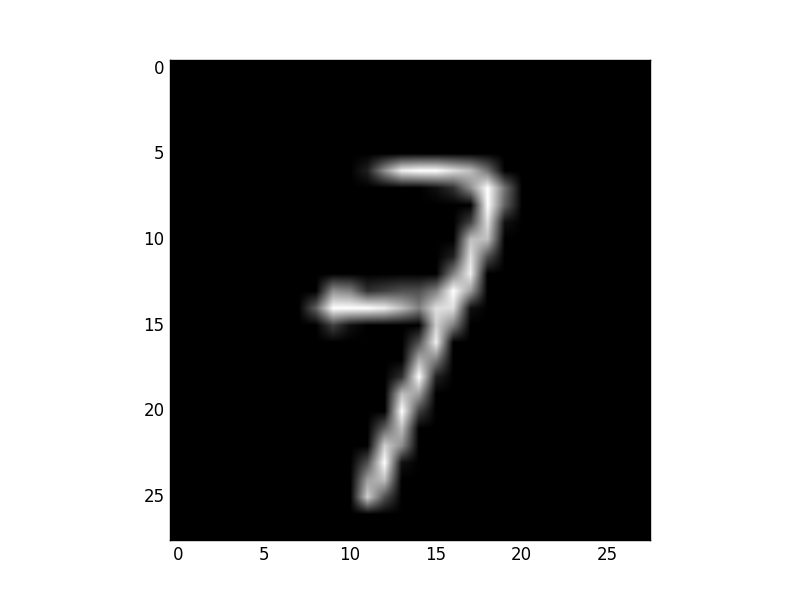
\includegraphics[height=1.2in]{figures/4_1_bad7}
        \caption{Misclassified 7}
    \end{subfigure}
    \caption{The MNIST dataset has some ambiguous entries, in accordance with real human handwriting, that are difficult to classify correctly.}
\end{figure}

\begin{table}[ht!]
\centering
\begin{tabular}{||c c c c c||}  
 \hline
 Dataset & LR Tr. & LR Test & SVM Tr & SVM Test \\ [0.3ex] 
 \hline\hline
 1 vs. 7 & 100.0 & 98.3 ($C=1$) & 100.0 & 98.7 ($C=0.2$) \\ 
 \hline
 3 vs. 5 & 100.0 & 93.3 ($C=60$) & 100.0 & 94.7 ($C=0.02$) \\ 
 \hline
 4 vs. 9 & 100.0 & 94.7 ($C=2$) & 100.0 & 94.7 ($C=0.02$) \\ 
 \hline
 odds vs. evens & 92.9 & 89.0 ($C=0.1$) & 93.9 & 89.2 ($C=0.02$) \\ 
 \hline
\end{tabular}
\caption{Accuracy of LR and Linear SVM on MNIST datasets.}
\label{table_4_1}
\end{table}

\subsection{Part 2}
Next, we applied the Gaussian RBF SVM classifier on the MNIST dataset for the same binary classification tasks.
Again, there are two parameters, $C$ (regularization) and $\gamma$ (bandwidth) that must be tuned with the validation set.
It is difficult to tune these two in parallel, especially without a method of visualizing the dataset, as was possible in the simple 2D data case.
Our approach was to train of each parameter in the range $[10^{-5}, 10^{-4}, ..., 10^{5}]$, and then compare accuracy on the validation set.
Many models had a validation accuracy of 99\%, so for these, the least complex model (low $\gamma$, low $C$).
Even so, it's very hard to select the best model because the relative importance of $C$ and $\gamma$'s size is not obvious (i.e. is a low $\gamma$ and high $C$ preferable to a high $\gamma$ and low $C$?).
The two are related to some extent; we observed roughly that an increase in order of magnitude of $\gamma$ decreases the $C$ for maximum validation accuracy, by an order of magnitude as well.
Also, $\gamma>1$ always has poor validation accuracy ($<60\%$) regardless of $C$.

The choice of $C$, $\gamma$, and training and test accuracy are shown in~\cref{table_4_2}.
Even with the poor choice of parameters in the stated range, validation accuracy was often around 70-80\%, so the classifier would not be completely useless.
For each classification task, the chosen hyperparameters are listed in~\cref{table_4_2}'s rightmost column.



[todo: compare rbf to linear classifiers]

\begin{table}[ht!]
\centering
\begin{tabular}{||c c c c||}  
 \hline
 Dataset & Tr. Acc & Test Acc & $C, \lambda$ \\ [0.3ex] 
 \hline\hline
 1 vs. 7 & 100.0 & 99.0 & 1, 0.01 \\ 
 \hline
 3 vs. 5 & 100.0 & 97.0 & 100, 0.001 \\ 
 \hline
 4 vs. 9 & 100.0 & 95.0 & 10, 0.001 \\ 
 \hline
 odds vs. evens & 100.0 & 97.2 & 1, 0.01 \\ 
 \hline
\end{tabular}
\caption{Accuracy of Gaussian RBF SVM classifier on MNIST datasets.}
\label{table_4_2}
\end{table}

\subsection{Part 3}
[todo]


%\listofchanges

%\balance

% \addtolength{\textheight}{-12cm} % This command serves to balance the column lengths
% on the last page of the document manually. It shortens
% the textheight of the last page by a suitable amount.
% This command does not take effect until the next page
% so it should come on the page before the last. Make
% sure that you do not shorten the textheight too much.

%%%%%%%%%%%%%%%%%%%%%%%%%%%%%%%%%%%%%%%%%%%%%%%%%%%%%%%%%%%%%%%%%%%%%%%%%%%%%%%%



%%%%%%%%%%%%%%%%%%%%%%%%%%%%%%%%%%%%%%%%%%%%%%%%%%%%%%%%%%%%%%%%%%%%%%%%%%%%%%%%



%%%%%%%%%%%%%%%%%%%%%%%%%%%%%%%%%%%%%%%%%%%%%%%%%%%%%%%%%%%%%%%%%%%%%%%%%%%%%%%%
% \section*{Acknowledgment}
% This work is supported by Ford Motor Company.
%%%%%%%%%%%%%%%%%%%%%%%%%%%%%%%%%%%%%%%%%%%%%%%%%%%%%%%%%%%%%%%%%%%%%%%%%%%%%%%%
%\clearpage
\balance
% \bibliographystyle{IEEEtran} 
% %\bibliographystyle{unsrt} 
% \bibliography{biblio}
% %\balance
\end{document}
%\grid
